\documentclass{article}\usepackage[]{graphicx}\usepackage[]{color}
%% maxwidth is the original width if it is less than linewidth
%% otherwise use linewidth (to make sure the graphics do not exceed the margin)
\makeatletter
\def\maxwidth{ %
  \ifdim\Gin@nat@width>\linewidth
    \linewidth
  \else
    \Gin@nat@width
  \fi
}
\makeatother

\definecolor{fgcolor}{rgb}{0.345, 0.345, 0.345}
\newcommand{\hlnum}[1]{\textcolor[rgb]{0.686,0.059,0.569}{#1}}%
\newcommand{\hlstr}[1]{\textcolor[rgb]{0.192,0.494,0.8}{#1}}%
\newcommand{\hlcom}[1]{\textcolor[rgb]{0.678,0.584,0.686}{\textit{#1}}}%
\newcommand{\hlopt}[1]{\textcolor[rgb]{0,0,0}{#1}}%
\newcommand{\hlstd}[1]{\textcolor[rgb]{0.345,0.345,0.345}{#1}}%
\newcommand{\hlkwa}[1]{\textcolor[rgb]{0.161,0.373,0.58}{\textbf{#1}}}%
\newcommand{\hlkwb}[1]{\textcolor[rgb]{0.69,0.353,0.396}{#1}}%
\newcommand{\hlkwc}[1]{\textcolor[rgb]{0.333,0.667,0.333}{#1}}%
\newcommand{\hlkwd}[1]{\textcolor[rgb]{0.737,0.353,0.396}{\textbf{#1}}}%
\let\hlipl\hlkwb

\usepackage{framed}
\makeatletter
\newenvironment{kframe}{%
 \def\at@end@of@kframe{}%
 \ifinner\ifhmode%
  \def\at@end@of@kframe{\end{minipage}}%
  \begin{minipage}{\columnwidth}%
 \fi\fi%
 \def\FrameCommand##1{\hskip\@totalleftmargin \hskip-\fboxsep
 \colorbox{shadecolor}{##1}\hskip-\fboxsep
     % There is no \\@totalrightmargin, so:
     \hskip-\linewidth \hskip-\@totalleftmargin \hskip\columnwidth}%
 \MakeFramed {\advance\hsize-\width
   \@totalleftmargin\z@ \linewidth\hsize
   \@setminipage}}%
 {\par\unskip\endMakeFramed%
 \at@end@of@kframe}
\makeatother

\definecolor{shadecolor}{rgb}{.97, .97, .97}
\definecolor{messagecolor}{rgb}{0, 0, 0}
\definecolor{warningcolor}{rgb}{1, 0, 1}
\definecolor{errorcolor}{rgb}{1, 0, 0}
\newenvironment{knitrout}{}{} % an empty environment to be redefined in TeX

\usepackage{alltt}

\usepackage{hyperref}

\title{Package \textbf{CompSign}}
\author{Lena Morrill}
\date{October 2017}
\IfFileExists{upquote.sty}{\usepackage{upquote}}{}
\begin{document}

\maketitle

\textbf{CompSign} is a package for yadayada... overlooked that mutational signatures are compositional in nature yadayada. The reference manual can be found \href{here}{https://github.com/lm687/CompSign/blob/master/CompSign.pdf}

\begin{knitrout}
\definecolor{shadecolor}{rgb}{0.969, 0.969, 0.969}\color{fgcolor}\begin{kframe}
\begin{alltt}
\hlcom{## knitr preferences}
\hlcom{## no chache}
\end{alltt}
\end{kframe}
\end{knitrout}

\begin{knitrout}
\definecolor{shadecolor}{rgb}{0.969, 0.969, 0.969}\color{fgcolor}\begin{kframe}
\begin{alltt}
\hlcom{## install latest version}
\hlkwd{library}\hlstd{(devtools)}
\hlstd{devtools}\hlopt{::}\hlkwd{install_github}\hlstd{(}\hlstr{"lm687/CompSign"}\hlstd{)}
\end{alltt}


{\ttfamily\noindent\itshape\color{messagecolor}{\#\# Skipping install of 'CompSign' from a github remote, the SHA1 (61cbadcb) has not changed since last install.\\\#\#\ \  Use `force = TRUE` to force installation}}\begin{alltt}
\hlkwd{library}\hlstd{(CompSign)}
\hlkwd{library}\hlstd{(compositions)}
\end{alltt}


{\ttfamily\noindent\itshape\color{messagecolor}{\#\# Loading required package: tensorA}}

{\ttfamily\noindent\itshape\color{messagecolor}{\#\# \\\#\# Attaching package: 'tensorA'}}

{\ttfamily\noindent\itshape\color{messagecolor}{\#\# The following object is masked from 'package:base':\\\#\# \\\#\#\ \ \ \  norm}}

{\ttfamily\noindent\itshape\color{messagecolor}{\#\# Loading required package: robustbase}}

{\ttfamily\noindent\itshape\color{messagecolor}{\#\# Loading required package: energy}}

{\ttfamily\noindent\itshape\color{messagecolor}{\#\# Loading required package: bayesm}}

{\ttfamily\noindent\itshape\color{messagecolor}{\#\# Welcome to compositions, a package for compositional data analysis.\\\#\# Find an intro with "{}? compositions"{}}}

{\ttfamily\noindent\itshape\color{messagecolor}{\#\# \\\#\# Attaching package: 'compositions'}}

{\ttfamily\noindent\itshape\color{messagecolor}{\#\# The following objects are masked from 'package:stats':\\\#\# \\\#\#\ \ \ \  cor, cov, dist, var}}

{\ttfamily\noindent\itshape\color{messagecolor}{\#\# The following objects are masked from 'package:base':\\\#\# \\\#\#\ \ \ \  \%*\%, scale, scale.default}}\end{kframe}
\end{knitrout}

\begin{knitrout}
\definecolor{shadecolor}{rgb}{0.969, 0.969, 0.969}\color{fgcolor}\begin{kframe}
\begin{alltt}
\hlcom{##########################}
\hlcom{####### Dummy data #######}
\hlcom{##########################}

\hlcom{### Example of matrix transformed into sign object}
\hlstd{input_dummy} \hlkwb{<-} \hlkwd{matrix}\hlstd{(}\hlkwd{runif}\hlstd{(}\hlnum{100}\hlstd{),} \hlnum{4}\hlstd{)}
\hlkwd{colnames}\hlstd{(input_dummy)} \hlkwb{<-} \hlkwd{paste0}\hlstd{(}\hlstr{'s'}\hlstd{,} \hlnum{1}\hlopt{:}\hlnum{25}\hlstd{);} \hlkwd{rownames}\hlstd{(input_dummy)} \hlkwb{<-} \hlkwd{paste0}\hlstd{(}\hlstr{'sam'}\hlstd{,} \hlnum{1}\hlopt{:}\hlnum{4}\hlstd{)}
\hlstd{sign_dummy} \hlkwb{<-} \hlkwd{to_sign}\hlstd{(input_dummy)}
\end{alltt}
\end{kframe}
\end{knitrout}

\section{Summarise the signature matrix}
\begin{knitrout}
\definecolor{shadecolor}{rgb}{0.969, 0.969, 0.969}\color{fgcolor}\begin{kframe}
\begin{alltt}
\hlkwd{add_together_matrix}\hlstd{(sign_dummy)}
\end{alltt}
\begin{verbatim}
## An object of class "sign"
## Slot "id":
## [1] "input_dummy"
## 
## Slot "id_samples":
## [1] "sam1" "sam2" "sam3" "sam4"
## 
## Slot "id_signatures":
##  [1] "s1"  "s2"  "s3"  "s4"  "s5"  "s6"  "s7"  "s8"  "s9"  "s10" "s11"
## [12] "s12" "s13" "s14" "s15" "s16" "s17" "s18" "s19" "s20" "s21" "s22"
## [23] "s23" "s24" "s25"
## 
## Slot "count_matrix":
##              s1         s2         s3        s4        s5         s6
## sam1 0.91779376 0.02385303 0.23876339 0.9712870 0.5408566 0.66646516
## sam2 0.01276465 0.34940536 0.63061196 0.6900336 0.3018326 0.60664123
## sam3 0.50539042 0.36147988 0.04297495 0.1056115 0.4906120 0.76086449
## sam4 0.70298904 0.03583288 0.65580700 0.4148143 0.5538498 0.07630959
##             s7        s8        s9        s10       s11       s12
## sam1 0.3374145 0.4773106 0.9515823 0.32474048 0.5656766 0.4174376
## sam2 0.9262440 0.7558482 0.6446747 0.54491706 0.5338909 0.8887019
## sam3 0.4919054 0.5217433 0.6016393 0.09456215 0.3792113 0.3280545
## sam4 0.8834992 0.1588780 0.4867555 0.19865778 0.3253180 0.3400624
##             s13        s14       s15       s16       s17       s18
## sam1 0.57315953 0.73772051 0.7100046 0.6773222 0.4430465 0.8818602
## sam2 0.82091263 0.49757104 0.7250833 0.7779467 0.8043129 0.3487173
## sam3 0.95243050 0.07723305 0.7091111 0.1253123 0.8933768 0.2195923
## sam4 0.09944258 0.17252315 0.4020018 0.2020037 0.2721947 0.3008867
##            s19         s20       s21       s22       s23       s24
## sam1 0.8509031 0.477927554 0.7759270 0.4968509 0.3611036 0.3978248
## sam2 0.3235608 0.008046405 0.2447500 0.5041135 0.3593709 0.2207983
## sam3 0.1355410 0.703507220 0.2849771 0.7882534 0.3600759 0.3927194
## sam4 0.8579977 0.757115631 0.3605919 0.8781320 0.8303557 0.4997538
##             s25
## sam1 0.11169879
## sam2 0.61510575
## sam3 0.78184170
## sam4 0.01722335
## 
## Slot "modified":
## [1] TRUE
\end{verbatim}
\begin{alltt}
\hlstd{results_sumarise} \hlkwb{<-} \hlkwd{summarise}\hlstd{(}\hlkwd{add_together_matrix}\hlstd{(sign_dummy))}
\hlstd{results_sumarise}\hlopt{$}\hlstd{General}
\end{alltt}
\begin{verbatim}
## [1] "Object of class sign"
\end{verbatim}
\end{kframe}
\end{knitrout}

\section{Linear model for numerical predictors}
\begin{knitrout}
\definecolor{shadecolor}{rgb}{0.969, 0.969, 0.969}\color{fgcolor}\begin{kframe}
\begin{alltt}
\hlstd{tmp_merged_compositional} \hlkwb{<-} \hlkwd{new}\hlstd{(}\hlstr{"merged_compositional"}\hlstd{,}
                                \hlkwc{id}\hlstd{=}\hlstr{'adas'}\hlstd{,}
                                \hlkwc{id_samples}\hlstd{=}\hlkwd{paste0}\hlstd{(}\hlstr{"sam"}\hlstd{,} \hlnum{1}\hlopt{:}\hlnum{30}\hlstd{),}
                                \hlkwc{id_signatures}\hlstd{=} \hlkwd{c}\hlstd{(}\hlstr{'s1'}\hlstd{,} \hlstr{'s2'}\hlstd{,} \hlstr{'s3'}\hlstd{,} \hlstr{'s4'}\hlstd{),} \hlcom{## signature names}
                                \hlkwc{count_matrix}\hlstd{=MCMCpack}\hlopt{::}\hlkwd{rdirichlet}\hlstd{(}\hlnum{30}\hlstd{,} \hlkwd{c}\hlstd{(}\hlnum{1}\hlstd{,}\hlnum{1}\hlstd{,}\hlnum{1}\hlstd{,}\hlnum{1}\hlstd{)),}
                                \hlkwc{df}\hlstd{=}\hlkwd{data.frame}\hlstd{(}\hlkwc{a}\hlstd{=}\hlkwd{sample}\hlstd{(}\hlnum{1}\hlopt{:}\hlnum{1e4}\hlstd{,} \hlnum{30}\hlstd{),} \hlkwc{b}\hlstd{=}\hlkwd{rep}\hlstd{(}\hlnum{10}\hlstd{,} \hlnum{30}\hlstd{)))}
\hlkwd{comp_lm}\hlstd{(tmp_merged_compositional)}
\end{alltt}
\begin{verbatim}
## [[1]]
## Response Y1 :
## 
## Call:
## lm(formula = Y1 ~ as.matrix((x@df)[, indices_predictor]))
## 
## Residuals:
##     Min      1Q  Median      3Q     Max 
## -2.9347 -0.6192  0.1741  0.8892  2.7811 
## 
## Coefficients: (1 not defined because of singularities)
##                                           Estimate Std. Error t value
## (Intercept)                             -2.794e-01  4.741e-01  -0.589
## as.matrix((x@df)[, indices_predictor])a  6.639e-05  7.658e-05   0.867
## as.matrix((x@df)[, indices_predictor])b         NA         NA      NA
##                                         Pr(>|t|)
## (Intercept)                                0.560
## as.matrix((x@df)[, indices_predictor])a    0.393
## as.matrix((x@df)[, indices_predictor])b       NA
## 
## Residual standard error: 1.333 on 28 degrees of freedom
## Multiple R-squared:  0.02614,	Adjusted R-squared:  -0.008636 
## F-statistic: 0.7517 on 1 and 28 DF,  p-value: 0.3933
## 
## 
## Response Y2 :
## 
## Call:
## lm(formula = Y2 ~ as.matrix((x@df)[, indices_predictor]))
## 
## Residuals:
##     Min      1Q  Median      3Q     Max 
## -3.1762 -0.8213 -0.0309  0.8489  2.9780 
## 
## Coefficients: (1 not defined because of singularities)
##                                           Estimate Std. Error t value
## (Intercept)                             -2.596e-02  5.195e-01  -0.050
## as.matrix((x@df)[, indices_predictor])a  1.697e-05  8.391e-05   0.202
## as.matrix((x@df)[, indices_predictor])b         NA         NA      NA
##                                         Pr(>|t|)
## (Intercept)                                0.960
## as.matrix((x@df)[, indices_predictor])a    0.841
## as.matrix((x@df)[, indices_predictor])b       NA
## 
## Residual standard error: 1.46 on 28 degrees of freedom
## Multiple R-squared:  0.001458,	Adjusted R-squared:  -0.0342 
## F-statistic: 0.0409 on 1 and 28 DF,  p-value: 0.8412
## 
## 
## Response Y3 :
## 
## Call:
## lm(formula = Y3 ~ as.matrix((x@df)[, indices_predictor]))
## 
## Residuals:
##      Min       1Q   Median       3Q      Max 
## -2.47089 -1.09373 -0.09707  0.98925  2.43186 
## 
## Coefficients: (1 not defined because of singularities)
##                                           Estimate Std. Error t value
## (Intercept)                              7.672e-01  4.930e-01   1.556
## as.matrix((x@df)[, indices_predictor])a -2.044e-04  7.963e-05  -2.566
## as.matrix((x@df)[, indices_predictor])b         NA         NA      NA
##                                         Pr(>|t|)  
## (Intercept)                               0.1309  
## as.matrix((x@df)[, indices_predictor])a   0.0159 *
## as.matrix((x@df)[, indices_predictor])b       NA  
## ---
## Signif. codes:  0 '***' 0.001 '**' 0.01 '*' 0.05 '.' 0.1 ' ' 1
## 
## Residual standard error: 1.386 on 28 degrees of freedom
## Multiple R-squared:  0.1904,	Adjusted R-squared:  0.1615 
## F-statistic: 6.586 on 1 and 28 DF,  p-value: 0.01591
\end{verbatim}
\end{kframe}
\end{knitrout}

\section{Importing data}
\begin{knitrout}
\definecolor{shadecolor}{rgb}{0.969, 0.969, 0.969}\color{fgcolor}\begin{kframe}
\begin{alltt}
\hlkwd{biplot}\hlstd{(}\hlkwd{princomp}\hlstd{(}\hlkwd{acomp}\hlstd{(MCMCpack}\hlopt{::}\hlkwd{rdirichlet}\hlstd{(}\hlnum{30}\hlstd{,} \hlkwd{rep}\hlstd{(}\hlnum{1}\hlstd{,} \hlnum{4}\hlstd{)))))}
\end{alltt}
\end{kframe}
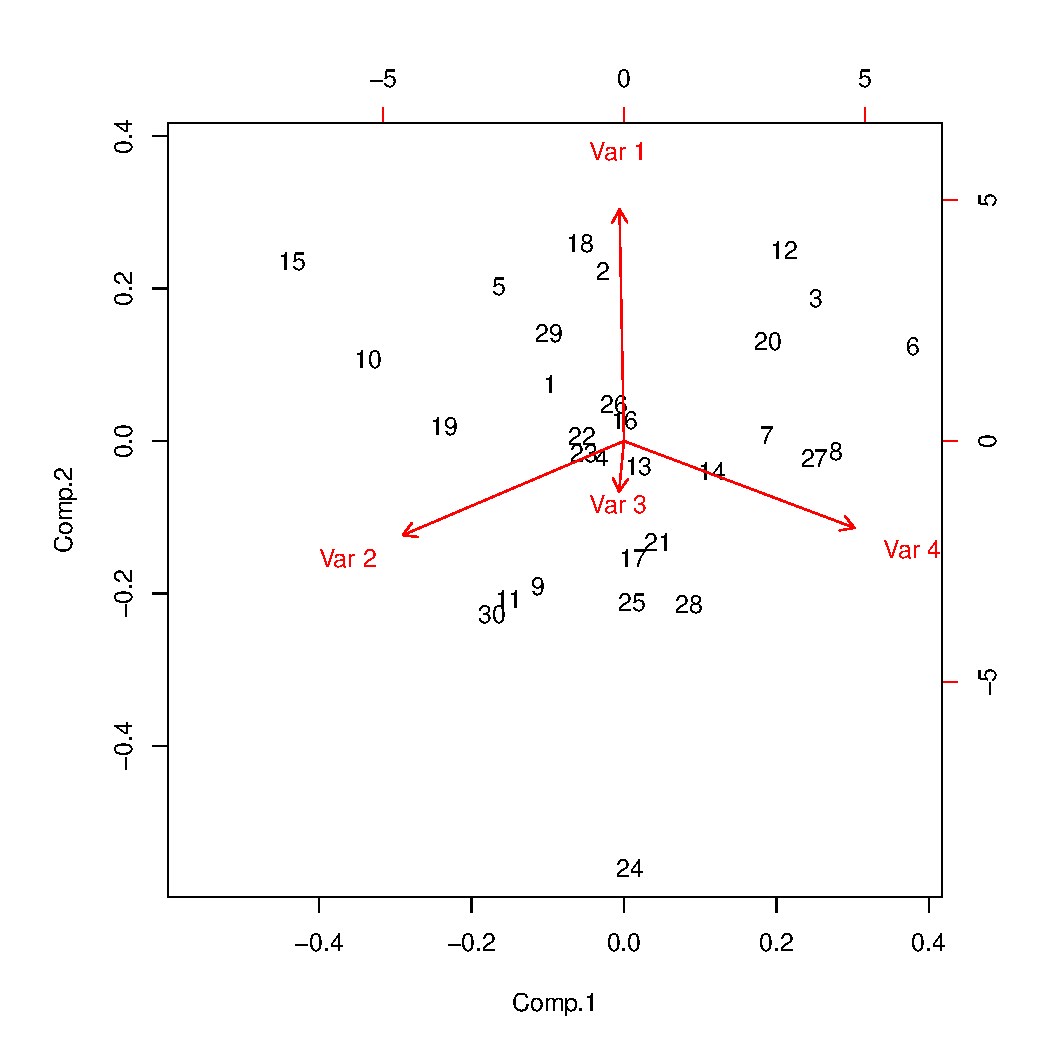
\includegraphics[width=\maxwidth]{figure/unnamed-chunk-6-1} 

\end{knitrout}

\section{Other}
\begin{enumerate}
\item Test for normality as follows:
\begin{knitrout}
\definecolor{shadecolor}{rgb}{0.969, 0.969, 0.969}\color{fgcolor}\begin{kframe}
\begin{alltt}
\hlkwd{data}\hlstd{(two_normal_pops)}
\hlkwd{par}\hlstd{(}\hlkwc{mfrow}\hlstd{=}\hlkwd{c}\hlstd{(}\hlnum{1}\hlstd{,}\hlnum{2}\hlstd{))}
\hlkwd{qqnorm.acomp}\hlstd{(}\hlkwd{acomp}\hlstd{(two_normal_pops}\hlopt{@}\hlkwc{count_matrix}\hlstd{),} \hlkwc{pch}\hlstd{=}\hlnum{19}\hlstd{,} \hlkwc{cex}\hlstd{=}\hlnum{0.2}\hlstd{)}
\end{alltt}
\end{kframe}
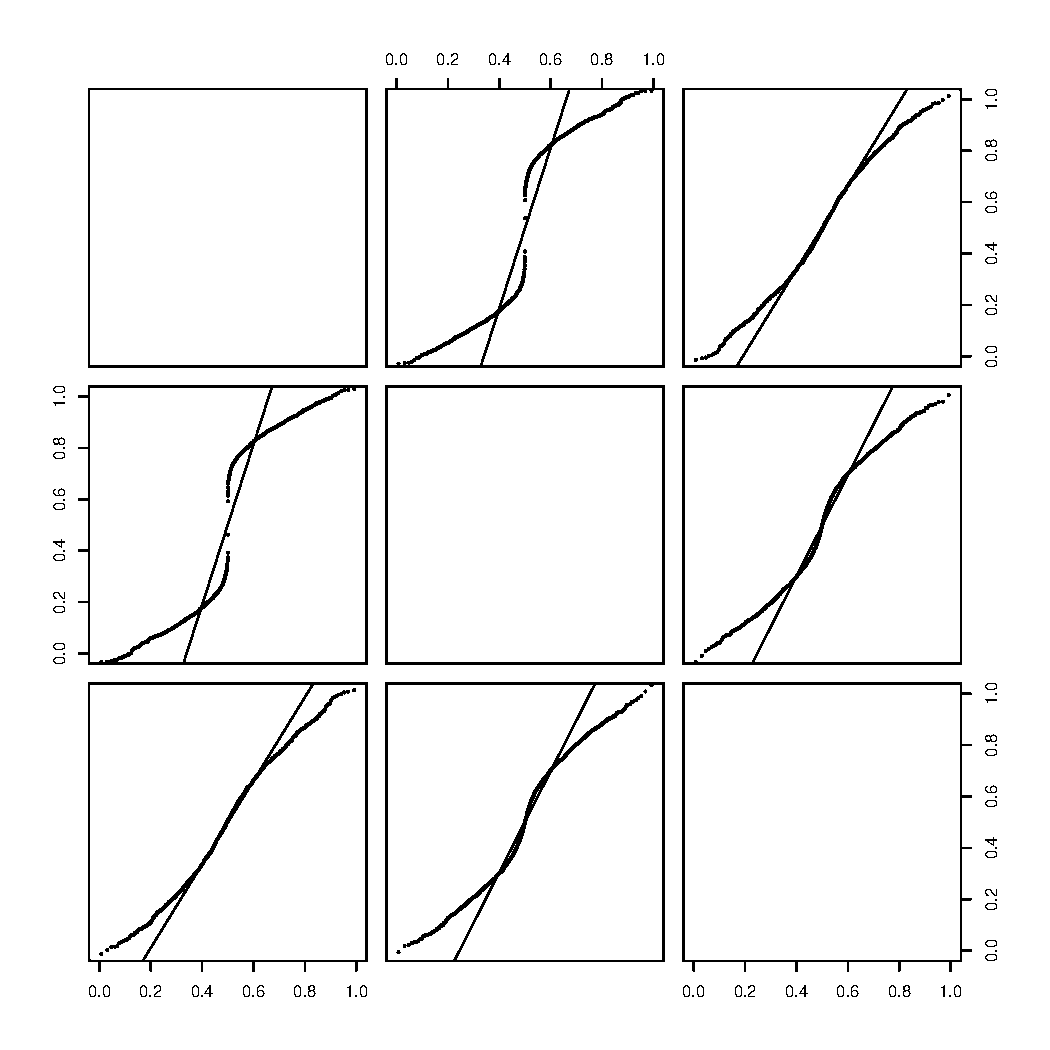
\includegraphics[width=\maxwidth]{figure/unnamed-chunk-7-1} 
\begin{kframe}\begin{alltt}
\hlkwd{qqnorm.acomp}\hlstd{(}\hlkwd{acomp}\hlstd{(two_normal_pops}\hlopt{@}\hlkwc{count_matrix}\hlstd{[}\hlnum{1}\hlopt{:}\hlnum{1000}\hlstd{,]),} \hlkwc{pch}\hlstd{=}\hlnum{19}\hlstd{,} \hlkwc{cex}\hlstd{=}\hlnum{0.2}\hlstd{)}
\end{alltt}
\end{kframe}
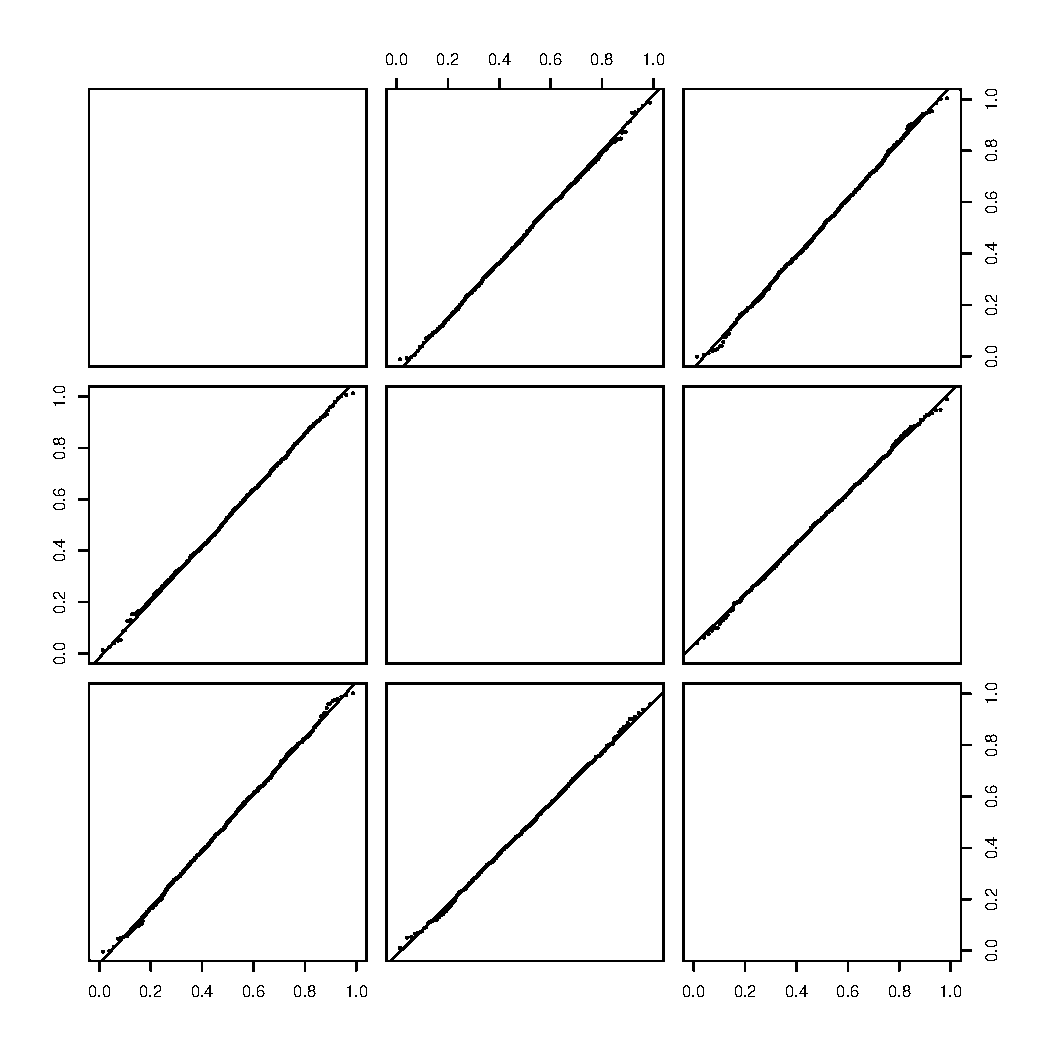
\includegraphics[width=\maxwidth]{figure/unnamed-chunk-7-2} 

\end{knitrout}
\end{enumerate}

\end{document}
